\documentclass[11pt]{article}
\usepackage{times}
\usepackage{amsfonts}
\usepackage{color}
\usepackage{multirow}
%\usepackage{rotating}
\usepackage{url}
\usepackage{latexsym}
\pagenumbering{arabic}
\usepackage{graphicx}
\title{Location-Based Dynamic Social Networks}


\author{
   Vladimir Eidelman, Raul Guerra, and Jim Stevens\\
Department of Computer Science \\
University of Maryland, College Park\\
   %\affaddr{College Park, MD 20742}\\
 { \tt \{vlad,rguerra,jims\}@cs.umd.edu}
}
\begin{document}

\maketitle 

\section{Introduction}


Technology, especially internet-based technology, has often been protrayed as having an alienating force by further removing us from `real' social interaction in favor of the virtual kind. However, a wave of recent applications has shown that in fact, the opposite can be true. Services such as Foursquare, Hot Potato, and Meetup have shown that we can actually enhance `real' experiences through the use of technology. 

In this paper, we present our efforts to extend that line of thinking in the form of location-based dynamic social networks. Imagine walking into a classroom or party, and having access to a dynamic social network with the other people in your immediate area, including desired profile information and real time information which is dependent on the venue. Motivated by the previous idea, the Proteus group implemented an application that generates dynamic networks that are location dependent for a user to immediately recognize people of interest or for a user to establish contact more easily with other users. The main objective is to facilitate interaction with new people around you who may potentially match your interests. The secondary objective is to find out if your friends are around and get together. 

The rest of this paper is structured as follows. First, we will present our overall system architecture in Section 2, including backend logic, database interaction, and user interfaces. Then, we will outline the implemented use cases in Section 3, followed by a discussion of future extensions in Section 4.


\section{System Architecture}

\subsection{Overview}

For the user, all interaction with the application takes place through a web interface. The first interaction users have is creating an account on the system. At this point, the user provides their profile information. This will also be used by the recommendation engine to match other users of interest. A user's profile resembles an online business card, only containing information they are willing to share with other people, since the emphasis is not in sharing personal information, but rather on encouraging real interaction. 

To complement the profile information, the user is constantly updating his or her context information. This includes active updates, where the user himself provides additional status information, like a list of interests, and passive updates, like location, where the users information is updated by the application automatically. The context information, in addition to the profile, is used by the application to find other users of interest. 

The interface interacts with a server to find other nearby users and, along with their context, displays the network of users logged in at a specific location in a Google Maps interface. Through the Google Map interface, the user can see other users' real time location, their profile information, links to other social media, such as Facebook and Twitter, and have an option to interact with them. 


As our application is web-based, it can run on any computer or mobile device which has a web browser, making it extremely portable. Making it light-weight in order not to unduly drain the limited resources of a mobile device was also a design priority, and thus all computation is performed on the servers, and only the necessary map update process runs on the device itself. 

However the application does need device specific information, the GPS location of the device running the application. This is not a problem because as the HTML5 standard becomes more pervasive, this application will be able to be deployed in any cellphone, PDA, iphones, etc. whose browser supports HTML5 geolocation capability.

%%diagram
Figure ~\ref{fig:arch} shows the structure of our system, as currently implemented. 
 
\begin{figure}[h]
\begin{center}
  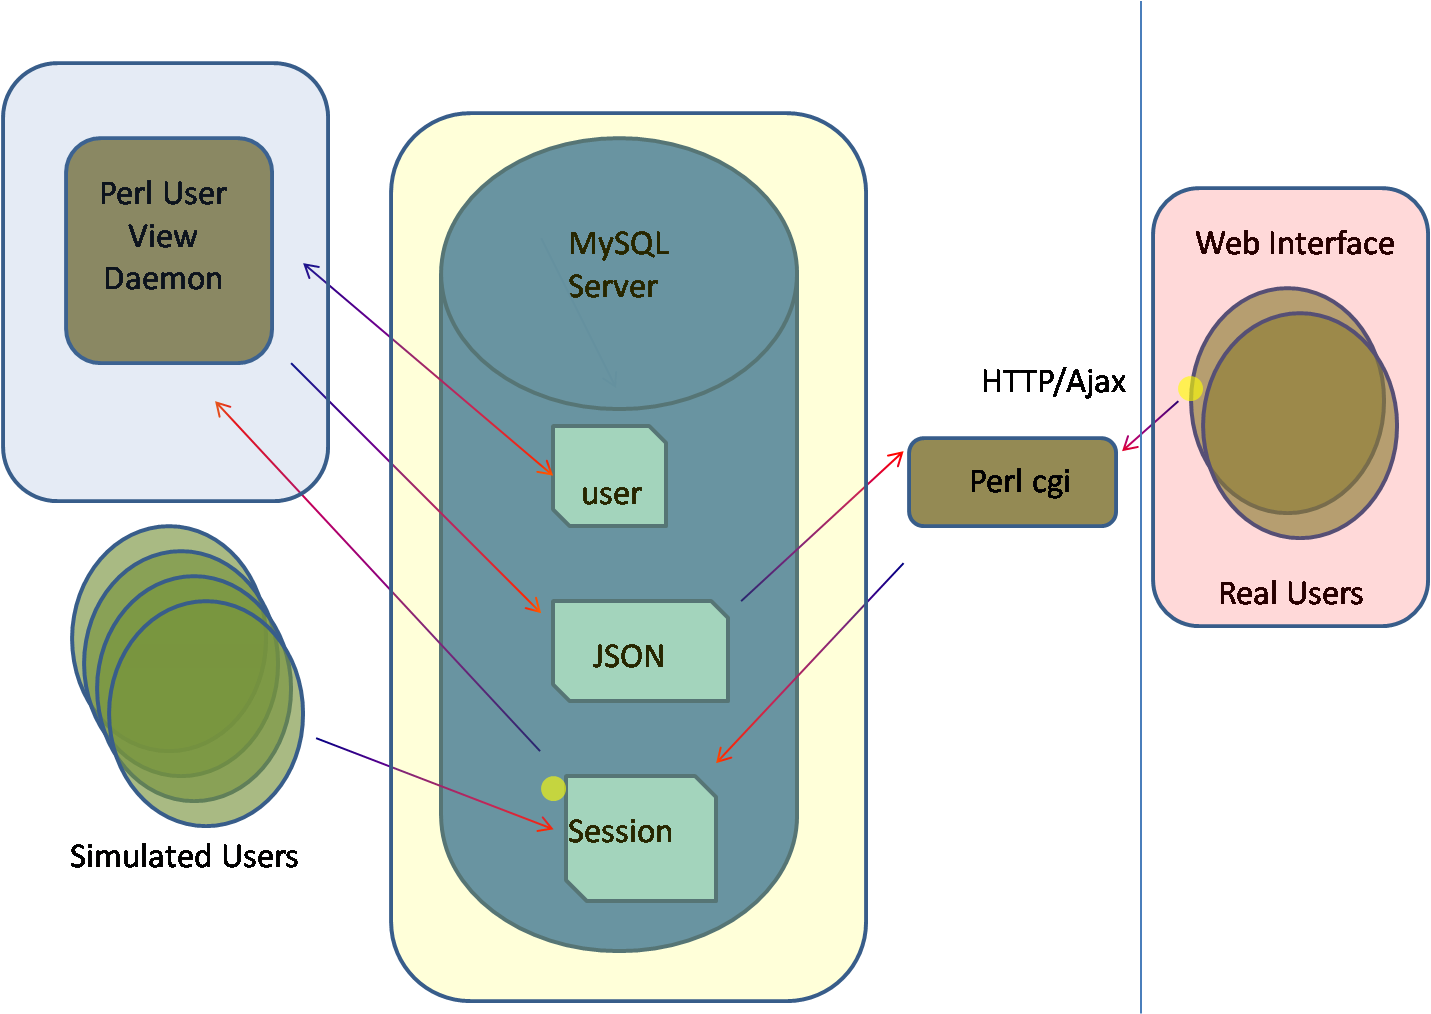
\includegraphics[scale=0.5]{sysarch.png}
\caption{System architecture}
\label{fig:arch} 
\end{center}
\end{figure}



\subsection{Database Setup}

%%database names and descriptions

While using the application, users will enter and leave the dynamic social network continuously, depending on whether a person is considered to be `present' in the network or not. To determine whether a person is considered to be `present', the application will use GPS information from the user's browser. 

\subsection{User Interaction}

%%user interface
Figure ~\ref{fig:phoneapp} shows the proposed interface for a mobile device.
 
\begin{figure}[h]
\begin{center}
  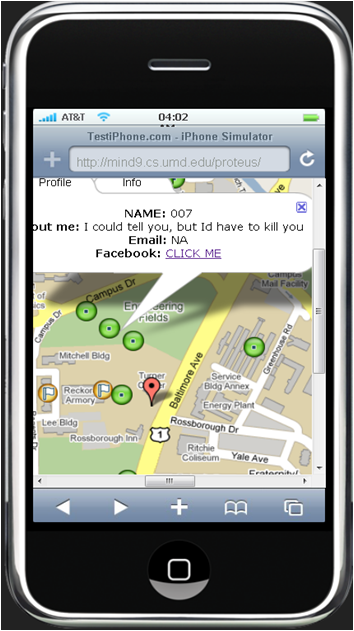
\includegraphics[scale=0.5]{phoneapp.png}
\caption{Example Apple iphone interface}
\label{fig:phoneapp} 
\end{center}
\end{figure}


The Google Map interface interacts with the backend both actively and passively. Actively, whenever a user wishes to query for other users in close proximity to himself, or post a Graffiti tag, the user submits his request to a CGI script written in Perl, which parses the query and performs the approrpriate action. Passively, while a user is logged into the system, the interface sends timed continuous updates indicating that the user is still active, and providing an updated locatin in the form of (longtitude, latitude), indicating the user should remain in the session table. In both cases, the script takes the information and inserts it into the appropriate places in the database. 

Then, the script asynchronously polls the JSON table, providing the map interface with the updated position, status, timestamp, etc. of the users which are in close proximity. 

\subsection{Google Mashup}

We currently support two different user interfaces, which we subsequently describe as location-based and name-based. The two views compliment each other in that the location view is useful for presenting a user with the layout of surrounding users, to encourage interaction with new peoepl in the immediately surrounding area, and the name view facilitates interacting with already known users. Figure ~\ref{fig:map1} presents the location view, which is the Google map interface that the user encounters upon logging into the system. 
Figure ~\ref{fig:userlist} presents a complimentary interface which allows users to scroll through a list of usernames to locate known friends.

Flags represent Graffiti tags.
Green dots represent users.

\subsection{Modularity}

%%how we can plug in/out fake users


\subsection{Daemon}


\section{Simulation}


In order to both validate the concept of our system and assess the structural limitations, we were inclined to design a simulation wherein we created virtual users. Utilizing the modularity described above, we were able to create an additional program which generated virtual users and updated their location, as if they were walking around campus, and plug it into our existing system as if the udpates were coming in from real users. 

The program generates 25 virutal users in random locations within College Park, along with their profile information, which includes emails and Facebook links. Then the program assigns one of 16 possible destinations for each user, and moves each user at a random reasonable rate toward their chosen destination, updating the appropriate tables in the database at the normal time intervals. The list of possible destinations includes itesm such as AV Williams, Stamp Student Union, the library, and downtown. Once a user reaches the assigned destination, a new one is chosen for them at random and the simulation proceeds. 

While the simulation is active, a real user can log into the sytem and interact with any one of the virtual users. Using the simulation provided us with a convenient way of presenting our vision for what the real application interface would feel like, as depicted in Figure~\ref{fig:sim1}. 


\begin{figure}[h]
\begin{center}
  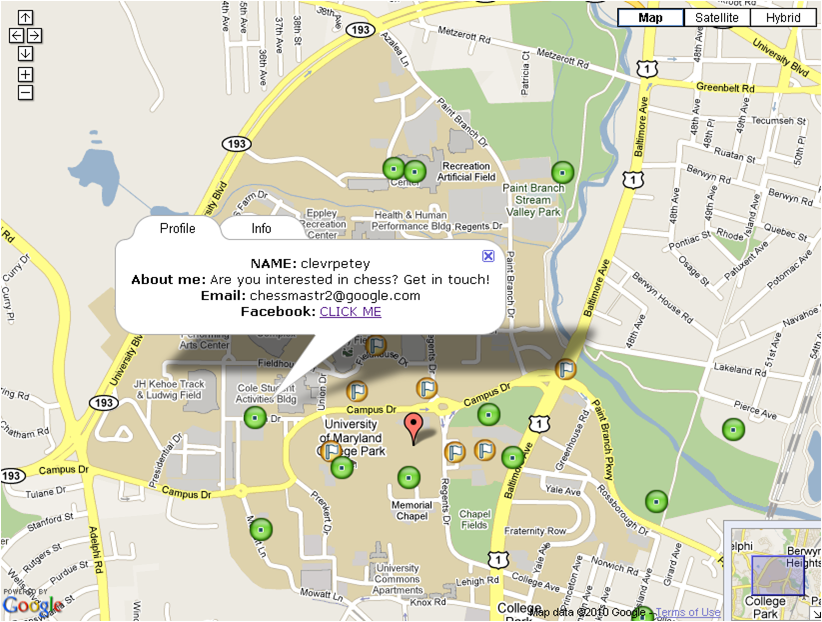
\includegraphics[scale=0.5]{sim1.png}
\caption{Example Apple iphone interface}
\label{fig:sim1} 
\end{center}
\end{figure}



\section{Future Work}
\subsection{Extensibility}

The project's biggest value resides both in the services it provides and the services it can be extended to provide, and the data it will produce once it is deployed. The application will produce a new type of social network data. While using the application, the users will be part of a complex social network which will be created and destroyed ad hoc in a short period of time. This will ellicit social interactions that do not happen in more rigid social networks like Facebook. This new type of data will raise questions in the area of Information Visualization, how can this rapidly changing data be best presented to a user? Machine Learning, how can this rapidly changing data be used by a learning system to infer information about the user? Can the application create surprise models based on this information. If the application becomes as widely used as other Social Networks, then more structural questions are raised. What other hardware should be added to a mobile device to extend the application's capabilities or to make the information handling faster? Networks, would other design structures (like peer-to-peer) improve the performance of the application?

By no means is the application limited only to facilitating social interactions. The application's capabilities can be extended to provide almost any service that is location dependent. 


Furthermore the application's services can be complemented by any information captured by sensors currently in and in future mobile devices by capturing the context around the user. This data can be used to better inform the server about a user's surroundings and for the server to make better inferences about the user's surroundings and make suggestions to the user. For instance, we see a strong potential for collaboration with the TagMeAr groups virtual reality application and our social network, in visualing the network and providing additional services.





Improve the way the server recommends users
Another potential is to export the interactions made in the application. For example, a user can keep track of who he or she talked to during an event, and after the event he or she can choose to keep a link through exporting it to a more permanent social networking. Then, using profile information and algorithms yet to be developed, we can decide how best to present the other members of the current dynamic networks to the user, so that they can see that they do know someone at the party, or that their friend is right next door having lunch.


\subsection{Graffiti/Tagging}
\subsection{Business Card/Profile}


{\color{red} 
{\it I dont think we should put it in this way, sounds to negative, like we didn't do anything, but I haven't modified it yet}
Currently the application only implements very general and simplified versions of the services previously described. In the current application, users can create an account with their profile information, and the only context information they provide is their real time location. Because of the limited context information, the user recommendation engine could not be implemented; there is not enough information to recommend one user over another. The Google Maps interface does show all the logged in users at a specific location moving in real time and allows a user to see other users' profile information and interact with them by writing in other users' walls. Future work would focus on the back end; implementing a recommendation engine;  making the application deployable; and making the application scalable.
}


 \section{Conclusion}


\end{document}



